%& -shell-escape
\documentclass[10pt,pdf,hyperref={unicode},xcolor=table]{beamer}

%\setbeamertemplate{background canvas}[vertical shading]
%%% Кордировка %%%
\usepackage[T2A]{fontenc}
\usepackage[utf8]{inputenc}
%\usepackage[document]{ragged2e}
\usepackage[russian,english]{babel}

%%% Математические пакеты %%%
\usepackage{amssymb,amsmath,mathtext,amsthm,amsfonts,amscd} % Математические дополнения от AMS

%%% Поддержка алгоритмов %%%
\usepackage[]{algorithm2e}
\usepackage{multirow}
%%% Изображения и графика %%%
\usepackage{graphicx}
\graphicspath{{./images/}}
\usepackage{cite,enumerate,float,indentfirst}
%\usepackage{lmodern}
%\usepackage{helvet}
%%% Поддержка комментариев %%%
\usepackage{verbatim}

%%% Схемы %%%
%\usepackage{tikz}

%%% Символы(галочка,...) %%%
\usepackage{amssymb}
\newcommand{\cmark}{\ding{51}}%


%%% Ссылки на локальные файлы %%%
\usepackage{hyperref}
%\usepackage{utopia}
%%% Доп св-ва таблиц %%%
%\usepackage[table,xcdraw]{xcolor}

% Выполнение комманд python из latex
\newcommand{\pyrun}[1]{\immediate\write18{#1.py}}
% 	Compile all the images from sources
%	\pyrun{plot-tree-regression}

% Красивое обозначение argmax, argmin
\DeclareMathOperator*{\argmin}{\arg\!\min}
\DeclareMathOperator*{\argmax}{\arg\!\max}

\newcommand{\B}[1]{\ensuremath{\mathbf{#1}}}
\newcommand{\rev}[1]{\frac{1}{#1}}
\newcommand{\e}{\mathop{\mathrm e}\nolimits}

\def\theme{Madrid}
\usecolortheme{whale}
	\usetheme{\theme}
	%\usefonttheme{default}
	\usefonttheme[onlymath]{serif}
	
	\title[Алгоритмы КЗ в антропометрии]{РАЗРАБОТКА И ПРИЛОЖЕНИЕ АЛГОРИТМОВ КОМПЬЮТЕРНОГО ЗРЕНИЯ К ЗАДАЧЕ АНТРОПОМЕТРИИ}
	\subtitle[кор. подназв.]{}
\author[Нгуен Тхе Лонг] % (optional)
{\bf{Нгуен Тхе Лонг}\\
Специальность 05.13.18  – Математическое моделирование, численные методы и комплексы программ\\
Научный руководитель: Профессор, д.ф.-м.н. Д.Н. Сидоров}
	

	
	\date[]{ Иркутск, 27 января 2017 г.} % (optional)
	
%%% Добавление номера страницы n/N %%%
\addtobeamertemplate{navigation symbols}{}{%
	\usebeamerfont{footline}%
	\usebeamercolor[fg]{footline}%
	\hspace{1em}%
	\insertframenumber/\inserttotalframenumber
}
%%% Установка цвета номера  %%%
\setbeamercolor{footline}{fg=black}

\newcommand{\citelink}[1] {
\cite{#1}\href{run:./materials/#1.pdf}{(link)}
}


\usepackage{pgfpages}
%\setbeameroption{show only notes}
%\setbeameroption{show notes}
%\setbeameroption{show notes on second screen=right}
\setbeamercolor{note page}{bg=white}
%\setbeamercolor{note title}{bg=gray}
\setbeamercolor{note date}{fg=white}

%------------------------------------------------------------
\begin{document}
\maketitle
\begin{frame}{Актуальность темы исследования}
\begin{block}{}
Диссертационное исследование позволяет решать прикладные задачи автоматизации антропометрии и относится к приоритетным направлениям научных исследований.
\end{block}
\begin{block}{}
В современной жизни устройства записи, обработки и воспроизведения цифровых изображений и видео высокого качества стали популярны для широкого круга пользователей.
\end{block}
\begin{block}{}
Возникают новые задачи, которые требует развития областей компьютерного зрения, чтобы получить доступ и эффективно создавать более интеллектуальные и более высокопроизводительные приложения.
\end{block} 
\begin{block}{}
Задача антропометрии требует привлечения научных инноваций, лучших методов, чтобы стать ближе к реальным потребностям в различных областях приложений антропометрии.
\end{block} 
\end{frame}
%-----------------------------------------------------------
\begin{frame}{}
\begin{block}{}
\textbf{Целью исследования} является применение численных методов компьютерного зрения и математического моделирования в антропометрии, реализация комплекса программ в виде приложения для смартфонов.
\end{block}
\begin{block}{}
\textbf{Задачи исследования:}
\begin{itemize}
	\item Разработка алгоритмов и методов компьютерного зрения для извлечения антропометрических признаков из изображений и видео в режиме реального времени при наличии шума;
	\item Объединение алгоритмов и методов компьютерного зрения для достижения высокой эффективности и повышения точности извлечения антропометрических признаков;
	\item Применение методов машинного обучения для классификации данных антропометрических признаков. Разработка метода построения антропометрической модели.
	\item Разработка антропометических приложений для смартфонов с операционной системой Андроид для использования в текстильной промышленности и в фитнесе;
	\item Оценка качества и эффективности работы системы компьютерного зрения в антропометрии на видео в среде Андроид.
\end{itemize}
\end{block}
\end{frame}
%-----------------------------------------------------------
\begin{frame}{Научная новизна}
\begin{block}{}
Предложены методы, алгоритмы компьютерного зрения для извлечения антропометрических признаков , основанные на сочетании двух алгоритмов сегментации изображения: разреза графов и алгоритма итеративных ближайших точек (Iterative Closest Point — ICP). Здесь цель состояла в том, чтобы получить полный набор ключевых точек, описывающих размеры человеческого тела;
\end{block}
\begin{block}{}
Приложение методов машинного обучения на основе случайного леса для классификации антропометрических измерений метода;
\end{block}
\begin{block}{}
Разработка методов построения антропометрических моделей человеческого тела на основе антропометрических признаков полученных при помощи авторских методов компьютерного зрения;
\end{block}
\begin{block}{}
Разработка бесконтактной системы антропометрии для смартфона на операционной системе Андроид.
\end{block}
		\end{frame}
%-----------------------------------------------------------
\begin{frame}{Внедрение работы и предмет исследования}
	\begin{block}{Внедрение работы}
Результаты исследования были применены на практике в области текстильной промышленности в компании «ШиК, ателье по пошиву военной формы» города Иркутска. Программа была представлена экспертам в этой области и были получены сертификаты, подтверждающие точность измерений и работоспособность приложения на практике.
	\end{block}
	\begin{block}{Предмет исследования}
Предмет исследования определен предметной областью №7 паспорта специальности 05.13.18 - «Разработка новых математических методов и алгоритмов интерпретации натурного эксперимента на основе его математической модели», а так же перечнем задач решаемых в диссертации.
	\end{block}
\end{frame}

%-----------------------------------------------------------
\begin{frame}{Методы исследования}
    \begin{block}{Методы теоретических исследований:}
			\begin{itemize}
         \item  Алгоритмы и методы компьютерного зрения в антропометрии;
				 \item  Методы анализа данных и построения 3D-моделей.
      \end{itemize}   
			\end{block}
				
		\begin{block}{Методы прикладных исследований:}
			\begin{itemize}
\item Проектирование алгоритмов для задачи извлечения признаков и классификации антропометрических признаков. Разработка 3D моделей для моделирования формы человеческого тела;
		\item Построение приложения на операционной системе Андроид;
		\item Тестирование программы и хранение результатов, оценка и сравнение результатов с другими методами и алгоритмами.
			\end{itemize}
    \end{block}
\end{frame}
%-----------------------------------------------------------
\begin{frame}{Теоретическая значимость и ценность исследования}
\begin{itemize}
	\item \textbf{Теоретической значимостью} результатов исследования диссертационной работы является разработка и тестирование новых моделей в антропометрии на основе сочетания алгоритмов и методов компьютерного зрения в антропометрии на основе обработки видеопотока.

\item \textbf{Исследования показали, что сочетание алгоритма сегментации изображений на основе разреза графов с  итеративным алгоритмом ближайших точек -  ICP повысило точность процесса извлечения антропометрических признаков. Кроме того, исследования показали, что алгоритм случайного леса позволяет эффективно решать задачу классификации антропометрических признаков.

\item \textbf{Практическая ценность} заключается в решении задачи антропометрии на базе смартфонов. Результаты внедрены для автоматизации процедуры профессионального снятия мерок для пошива одежды, а также для фитнес-тестирования.
 \end{itemize}
\end{frame}
%------------------------------------------------------------
\begin{frame}
	\begin{columns}
		\begin{column} {0.5\textwidth}		
			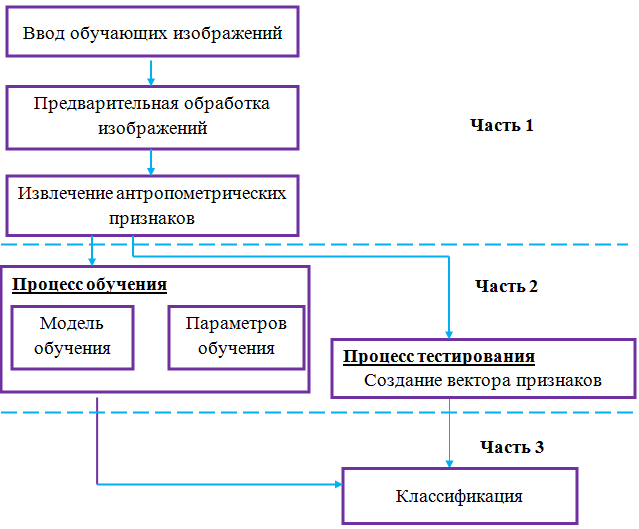
\includegraphics[width=1\linewidth]{p1}
			\end{column}
			\begin{column} {0.5\textwidth}
				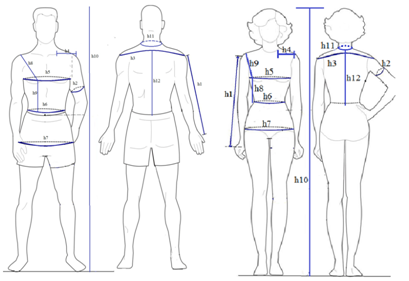
\includegraphics[width=1\linewidth]{p2}
			\end{column}      
		\end{columns}
\begin{block}{Описание системы антропометрии на основе компьютерного зрения}
			\begin{itemize}
\item Часть 1 - Извлечение антропометрических признаков на основе методов компьютерного зрения;
\item Часть 2 - Классификация данных векторов антропометрических признаков на основе методов машинного обучения;
\item Часть 3 - Построение антропометрической модели.
\end{itemize}
		\end{block}
\end{frame}
%-----------------------------------------------------------
\begin{frame}{Обнаружение объектов}
\begin{columns}
		\begin{column} {0.5\textwidth}			
			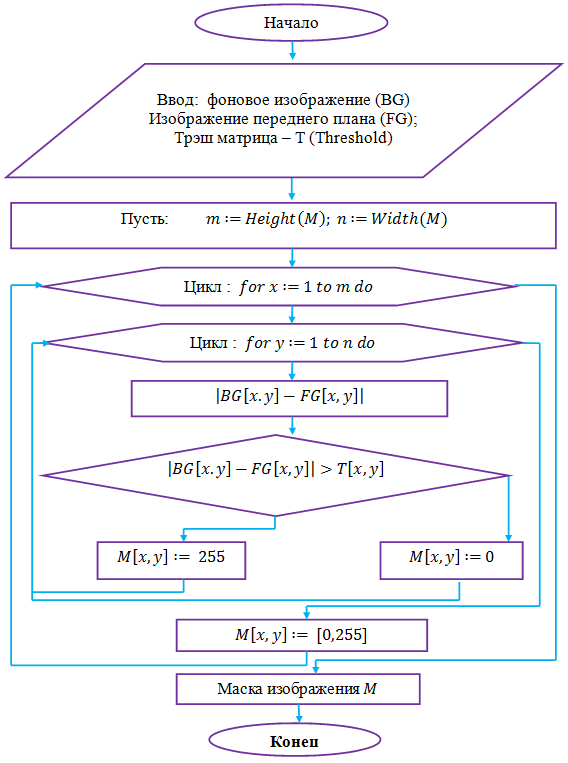
\includegraphics[width=1\linewidth]{p3}
			\end{column}
			\begin{column} {0.5\textwidth}
						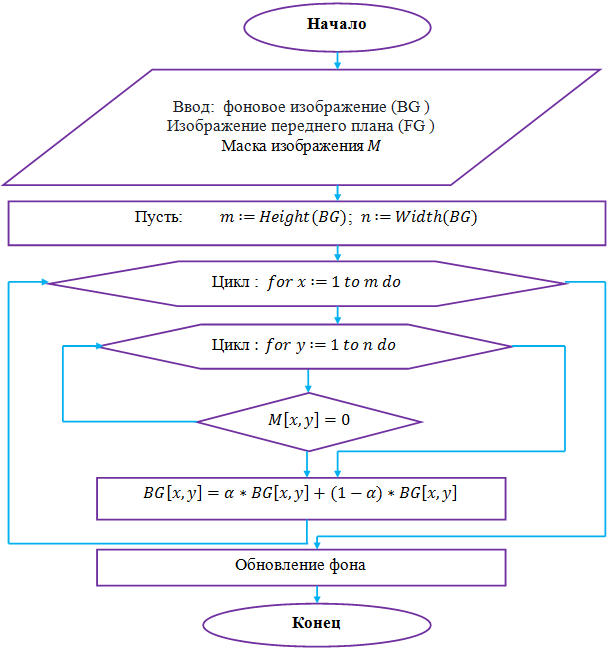
\includegraphics[width=1\linewidth]{p4}
			\end{column}      
		\end{columns}
\end{frame}
%%%%%%%%%%%%%%%%5
%-----------------------------------------------------------
\begin{frame}{Сегментация изображения алгоритмом разреза на графах}		
\begin{columns}
		\begin{column} {0.4\textwidth}			
			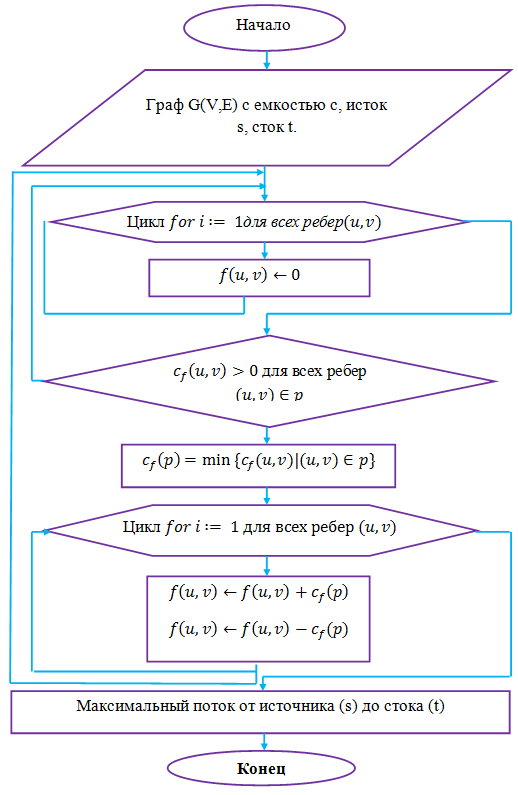
\includegraphics[width=1\linewidth]{p5}
			\end{column}
			\begin{column} {0.6\textwidth}
			\begin{block}{}
			\begin{itemize}
	\item $f\left(u,v\right) \leq c\left(u,v\right)$ - Это поток из u в v не превосходит пропускной способности;
	\item $f\left(u,v\right) =-f\left(v,u\right)$;
	\item $\sum_vf\left(u,v\right)=0 \leftrightarrow f_{in}\left(u\right) =f_{out}\left(v\right)$ для всех узлов $u$, кроме $s$ и $t$;

	\item Остаточная сеть $G_f\left(V,E_f\right)$ - сеть с  пропускной способностью $c_f\left(u,v\right)=c\left(u,v\right)-f\left(u,v\right)$ и без потока Ford – Fulkerson (1956).
\item $E\left(f\right) = \sum_{p \in P}D_p\left(f_p\right)+\sum_{p,q \in N}V_{p,q}\left(f_p,f_q\right)$
\item Найти маркировки $f:P\rightarrow L$ , что сводит к минимуму $E\left(f\right)$ из множеств пикселей $P$, набор этикеток $L,N \in P$ является система соседства по пикселям. 
	\end{itemize}
	\end{block}
			\end{column}      
		\end{columns}
	
\end{frame}
%%%%%%%%%%%%%%%%5
\begin{frame}{Итеративный алгоритм ближайших точек}		
\begin{columns}
		\begin{column} {0.4\textwidth}			
			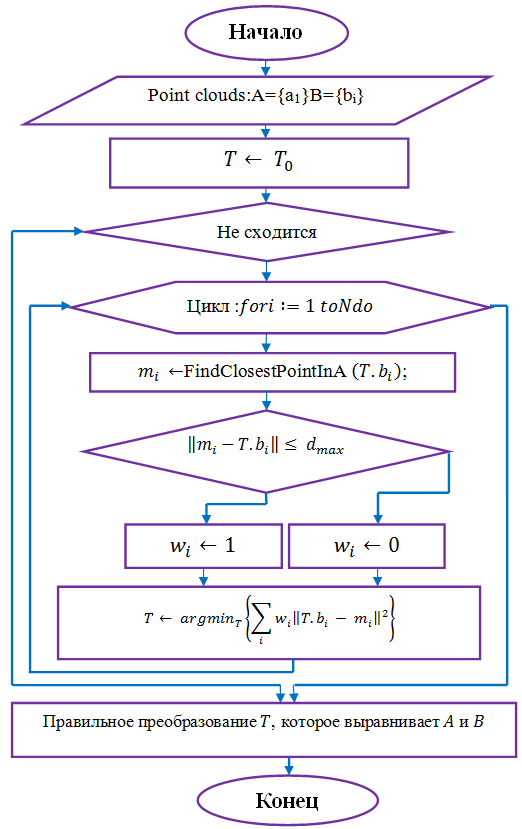
\includegraphics[width=1\linewidth]{p6}
			\end{column}
			\begin{column} {0.6\textwidth}
			\begin{block}{}
	\begin{itemize}
	\item \textbf{Шаг 1:} Вычислим соответствия между двумя сканированиями;
	\item \textbf{Шаг 2:} Выполним преобразование, которое сводит к минимуму расстояние между соответствующими точками.
\end{itemize}
	\end{block}
	Алгоритм $ICP$ повторяет действия, чтобы минимизировать среднеквадратичную ошибку.
$ T\leftarrow argmin_t\left\{\sum_i\left\|T.b_i - m_i\right\|^2\right\}$\\
Где:
\begin{itemize}
	\item $T$ - правильное преобразование;
	\item $b_i$: $B=\left\{b_i\right\}$ - облако точек;
	\item $m_i$ - множество точек, которые будут преобразованы из $B$ - $A$ ( $A=\left\{a_i\right\}$ - облако точек);
\end{itemize}
			\end{column}      
		\end{columns}	
\end{frame}
%%%%%%%%%%%%%%%%5
\begin{frame}{Общая блок-схема процесса системы}		
\begin{columns}
		\begin{column} {0.5\textwidth}			
			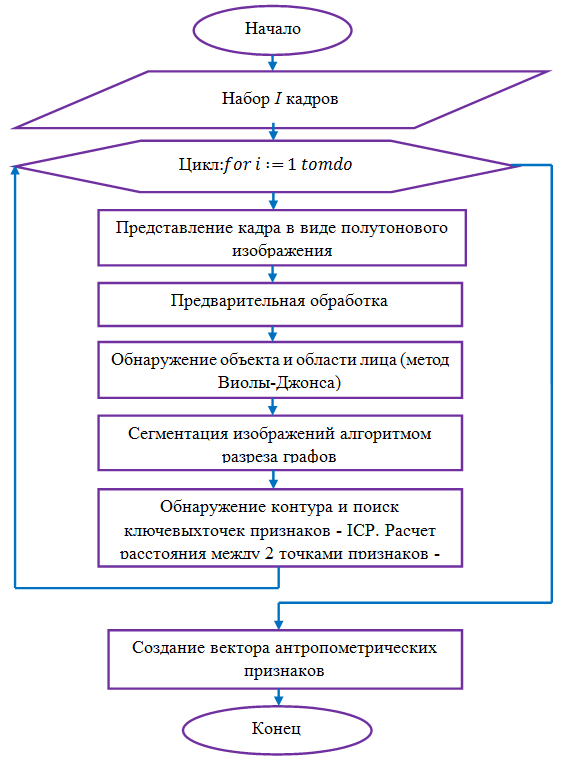
\includegraphics[width=1\linewidth]{p7}
			\end{column}
			\begin{column} {0.5\textwidth}
			\begin{block}{}
	\textbf{Шаг 1:}Предварительная обработка изображения;
	\end{block}
				\begin{block}{}
\textbf{Шаг 2:}Обнаружение объекта и человеческого лица.
\end{block}
\begin{block}{}
	 \textbf{Шаг 3:}Сегментация изображения методом разреза на графах;
\end{block}
\begin{block}{}
	\textbf{Шаг 4:}Обнаружение контура и поиск ключевых точек признаков – алгоритм $ICP$. Расчет евклидова расстояния: $d\left(A,B\right) = \sqrt{\left(x_B - x_A\right)^2 + \left(y_B - y_A\right)^2}$;
	\end{block}
	\begin{block}{}
	\textbf{Шаг 5:}Создание антропометрического вектора признаков.
\end{block}
			\end{column}      
		\end{columns}	
\end{frame}
%%%%%%%%%%%%%%%%5
\begin{frame}{Результат обработки изображений}		
\begin{columns}
		\begin{column} {0.8\textwidth}
\begin{table}[b!]%	
		\begin{tabular}{|c|c|c|c|c|}
    \hline
    \multirow{2}{*}{Антропометрические} & {Ручной} & \multicolumn{3}{c}{Результаты системы} \\
      признаки & метод  &1 &2 &3 \\
    \hline
Грудь             &95	&95.03	&95.00	&95.02	\\
\hline 
Талия             &79	&78.46	&79.05	&78.89 \\

\hline
Бедра               &96.5	&97.29	&96.11	&96.4\\

\hline
Длина рук           &53	&52.93		&52.1	&52.93\\

\hline
Обхват бицепса      &28	&28.24	&28.03	&28.07\\

\hline
Обхват шеи         &37	&38.35	&38.13	&38.05	\\

\hline
Длина спины         &40	&38.35	&39.96	&39.81	\\

\hline
Длина плеча       &36	&36.01	&36.17	&36.1	\\

\hline
Ширина плеча        &14	&13.97	&14.02	&14.02	\\

\hline
Высота груди       &18	&18.05	&18.11	&18.01 \\

\hline
  \end{tabular}
\end{table}
		\end{column}
			\begin{column} {0.2\textwidth}	
			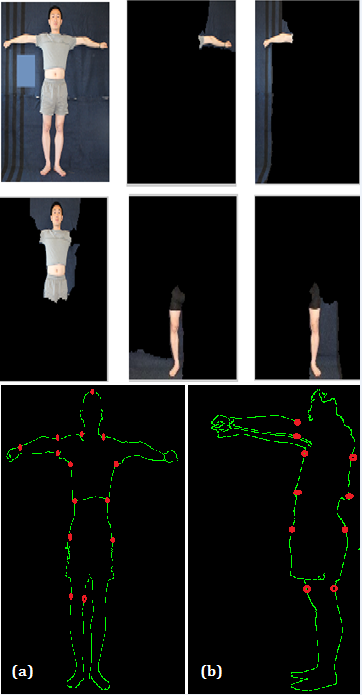
\includegraphics[width=1\linewidth]{p9}
					\end{column}      
		\end{columns}	
		
		\begin{center}
		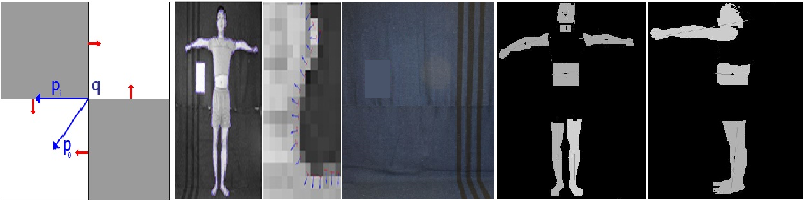
\includegraphics[width=0.7\linewidth]{p8}
		\end{center}
		
\end{frame}
%%%%%%%%%%%%%%%%5
\begin{frame}{Оценивание точности метода извлечения антропометрических признаков}		
\begin{columns}
		\begin{column} {0.6\textwidth}			
\begin{block}{}
$MAPE$:
$ M=\frac{1}{n}\sum^n_{i=1}\left|\frac{A_t-F_t}{A_t}\right|$
Где:
\begin{itemize}
	\item $A_t$: Результат измерений, рассчитанных вручную;
	\item $F_t$: Результат извлечения антропометрических признаков.
\end{itemize}
\end{block}

\begin{center}
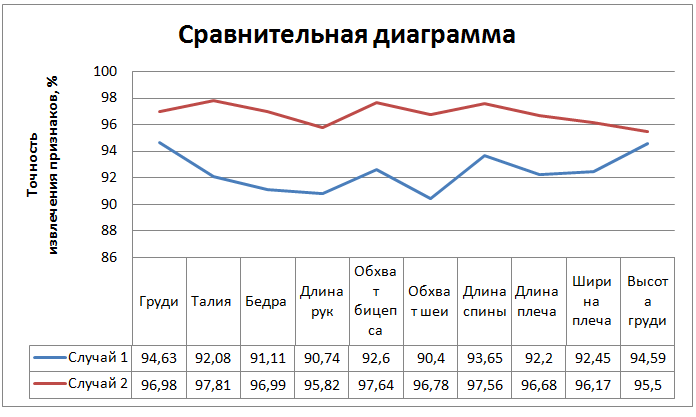
\includegraphics[width=0.9\linewidth]{p11}
\end{center}

			\end{column}
			\begin{column} {0.4\textwidth}
		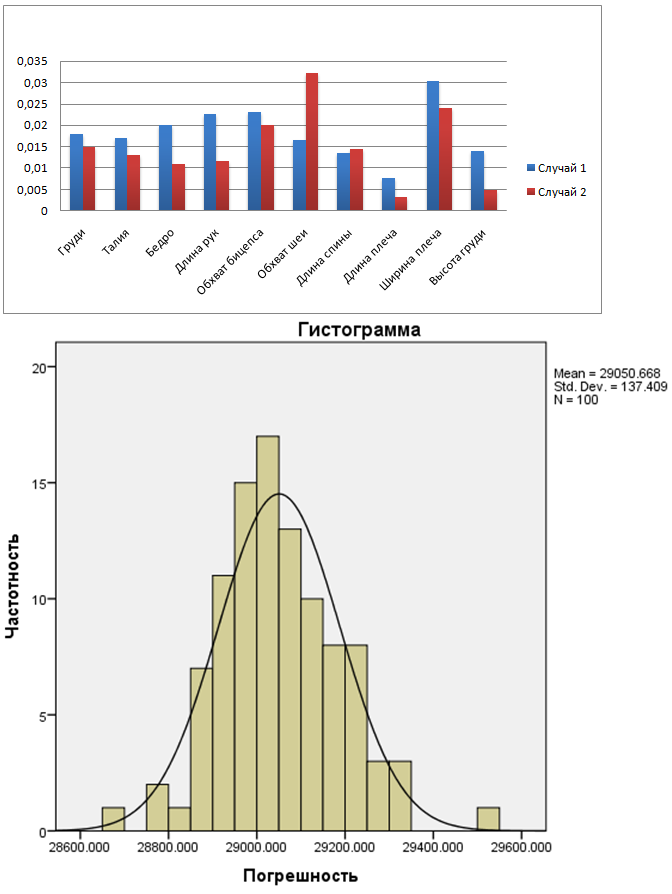
\includegraphics[width=0.9\linewidth]{p10}
			\end{column}      
		\end{columns}
\end{frame}
%%%%%%%%%%%%%%%%5
\begin{frame}{Применение алгоритма Random Forest для классификации антропометрических данных}
\begin{columns}
		\begin{column} {0.7\textwidth}			
\begin{itemize}
	\item \textbf{Шаг 1:} Создание $m$ наборов признаков из $n$ наборов первоначальных признаков. Каждый набор содержит $2 \frac{n}{m} $признаки. 	
	\item \textbf{Шаг 2:} Использование Random Forest для того, чтобы вычислять оценку наборов признаков $\Rightarrow$ получение набора значений $f\left(i\right), i= \left(1,..., m\right)$;
	\item \textbf{Шаг 3:}взвешивание каждого признака $i$ рассчитывается по формуле:
	$w_j= \sum^m_{i=1}kf_i$;	
	\item \textbf{Шаг 4:} Разработка нового признака включает в себя $р\%$ лучших признаков;
	\item \textbf{Шаг 5:} Повторение шага $1$ для удовлетворения одного из двух условий: Количество признаков < порога разрешено; Количество циклов определено.
	
\end{itemize}

			\end{column}
			\begin{column} {0.3\textwidth}
		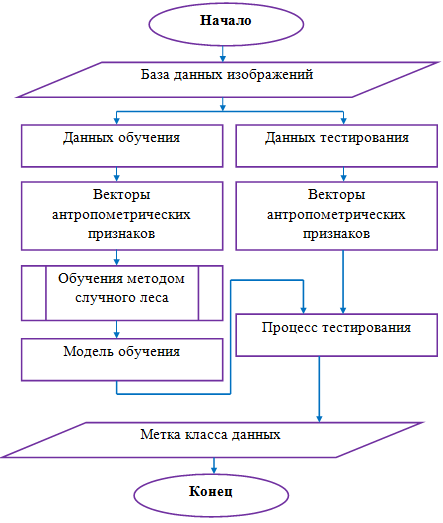
\includegraphics[width=1\linewidth]{p12}
			\end{column}      
		\end{columns}
\end{frame}

%%%%%%%%%%%%%%%%5
\begin{frame}{Основные этапы подготовки данных}
\begin{columns}
		\begin{column} {0.7\textwidth}			
\begin{itemize}
	\item Шаг 1: Описание текстурных характеристик человеческого тела (кожа, волосы, лицо), текстуры одежды;
   \item Шаг 2: Идентификация частей человеческого тела (голова, туловище, руки, ноги) и их антропометрических признаков;
\item Шаг 3: Объединение текстур и частей человеческого тела в блок;
\item Шаг 4: Экспорт 3D модели человеческого тела в два файла: файлы текстуры и файлы, содержащие информацию каждой модели.
\end{itemize}

			\end{column}
			\begin{column} {0.3\textwidth}
		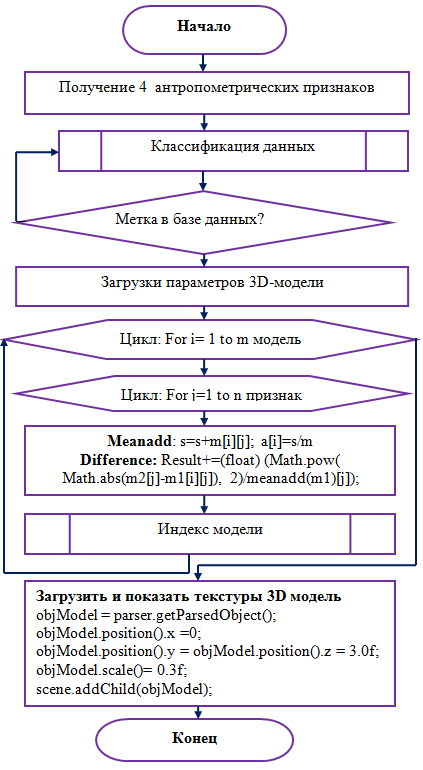
\includegraphics[width=1\linewidth]{p13}
			\end{column}      
		\end{columns}
\end{frame}
%%%%%%%%%%%%%%%%5
\begin{frame}{Результаты построения 3D моделей}
\begin{block}{}
$ Model = Min\left\{\sum^N_{i=1}\left(B-B_i\right)^2+\left(C-C_i\right)^2+\left(W-W_i\right)^2+\left(H-H_i\right)^2\right\}$
\end{block}	
\begin{table}[b!]%
\begin{center}
  \begin{tabular}{|c|c|c|c|c|}
    \hline
  Количество  & Среднее   &   Стандартное   & Минимальное   & Максимальное \\
деревьев     & значение  &    отклонение   & значение      &значение      \\
\hline
100	&0.0116	&0.00833	&0.00463	&0.0202\\
\hline
200	&0.0092	&0.00667	&0.00516	&0.0117 \\
\hline
300	&0.02178	&0.00416	&0.0040	&0.0221\\
\hline
400	&0.00726	&0.0050	&0.0071	&0.009\\
\hline
500	&0.00553	&0.00383	&0.00513	&0.0085\\
\hline
  \end{tabular}
\end{center}
\end{table}%\vspace{10mm}

\begin{center}
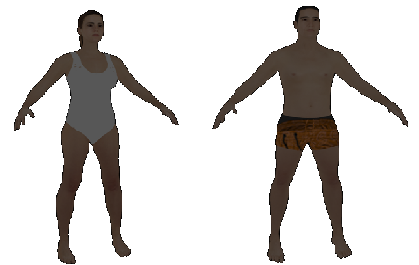
\includegraphics[width=0.45\linewidth]{p14}
\end{center}

\end{frame}
%-----------------------------------------------------------
\begin{frame}{Анализ и проектирование системы компьютерного зрения в антропометрии}
\begin{block}{Диаграмма прецедентов и диаграмма классов E-Tailor}
Система имеет основные функции:
\begin{itemize}
	\item Сбор данных с камеры;
	\item Заполнение информации о росте, весе;
	\item 3D-моделирование человеческого тела;
	\item Классификация и предсказание размеров одежды;
	\item Контакты с командой разработчиков.
\end{itemize}
\end{block}
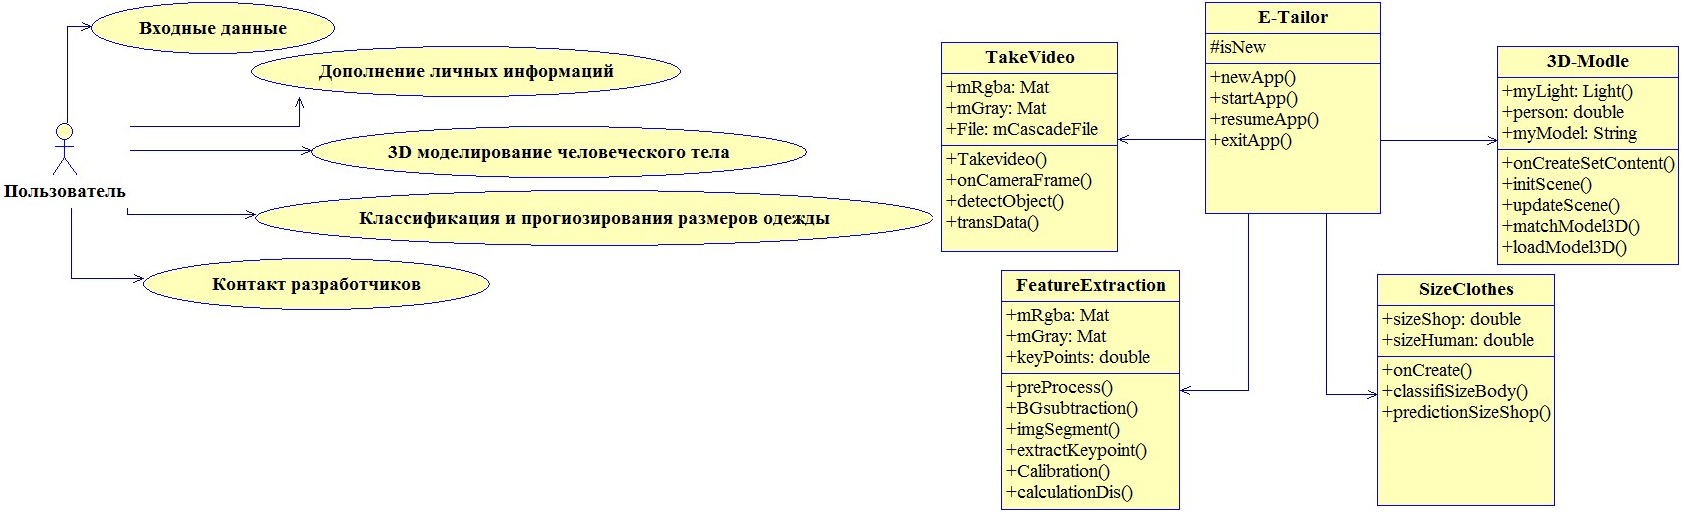
\includegraphics[width=1\linewidth]{p15}
\end{frame}
%-----------------------------------------------------------
\begin{frame}{}
\begin{figure}[ht!]
\centering
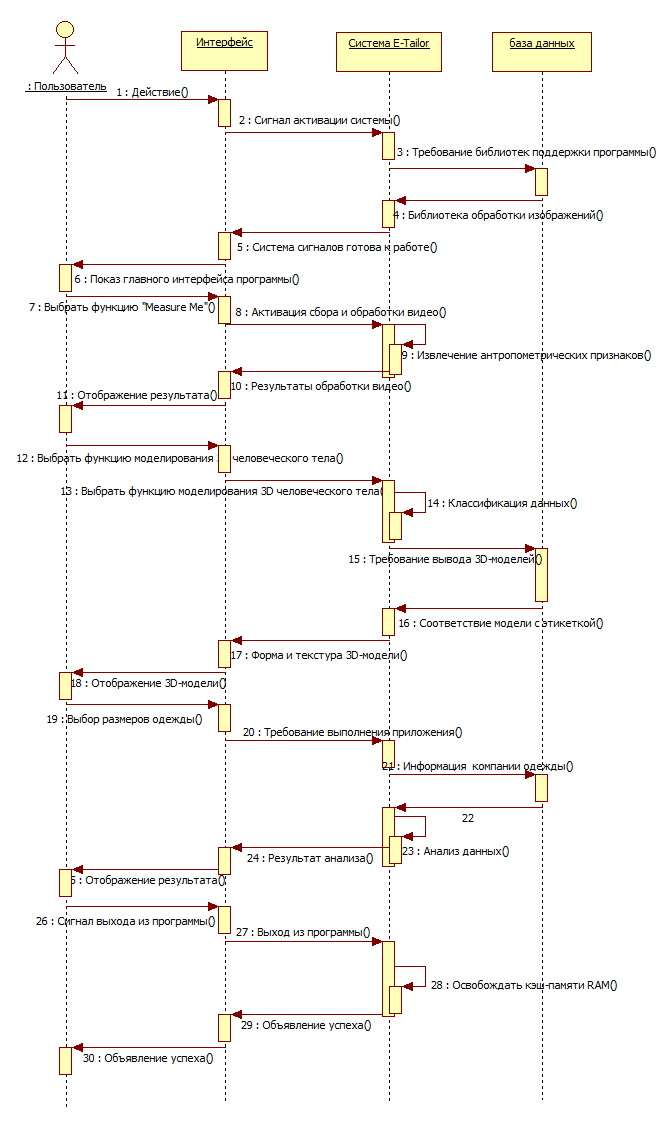
\includegraphics[width=0.45\linewidth]{p16}
\begin{center}
%\captionsetup{justification=justified, labelsep=period}
\caption{Диаграмма последовательности - система компьютерного зрения в антропометрии приложения E- Tailor.}
\end{center}
\end{figure}
\end{frame}
%-----------------------------------------------------------
\begin{frame}{Диаграмма прецедентов и диаграмма классов E-Fitness}
\begin{columns}
		\begin{column} {0.5\textwidth}			
Система имеет основные функции:
\begin{itemize}
	\item Сбор данных с камеры;
	\item Заполнение информации о росте, весе;
	\item 3D-моделирование человеческого тела;
	\item Анализ антропометрических признаков по стандартам фитнеса;
	\item Анализ ожирения в соответствии с индексом ИМТ;
	\item Тренажерные упражнения фитнеса в домашних условиях;
	\item Контакты с командой разработчиков.
\end{itemize}
			\end{column}
			\begin{column} {0.5\textwidth}
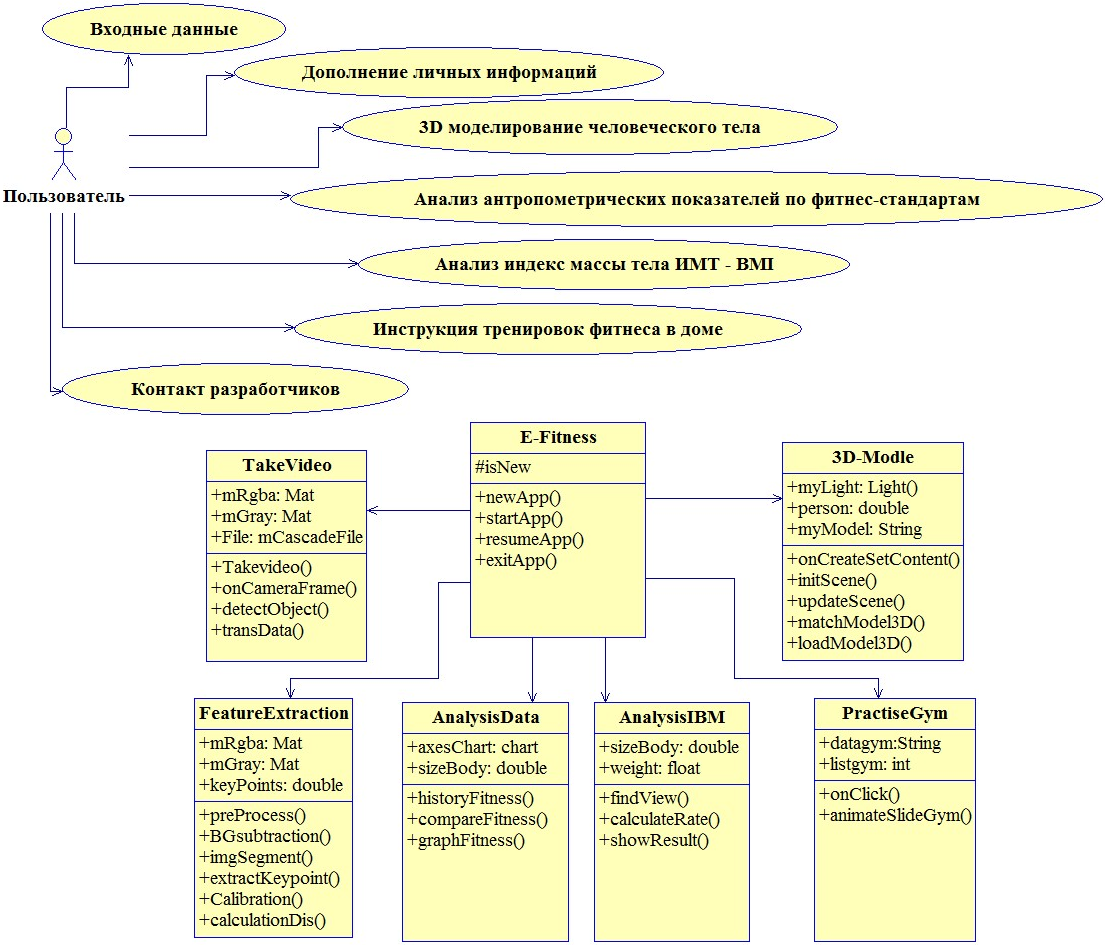
\includegraphics[width=1\linewidth]{p17}
			\end{column}      
		\end{columns}
\end{frame}
%-----------------------------------------------------------
\begin{frame}{}
\begin{figure}[ht!]
\centering
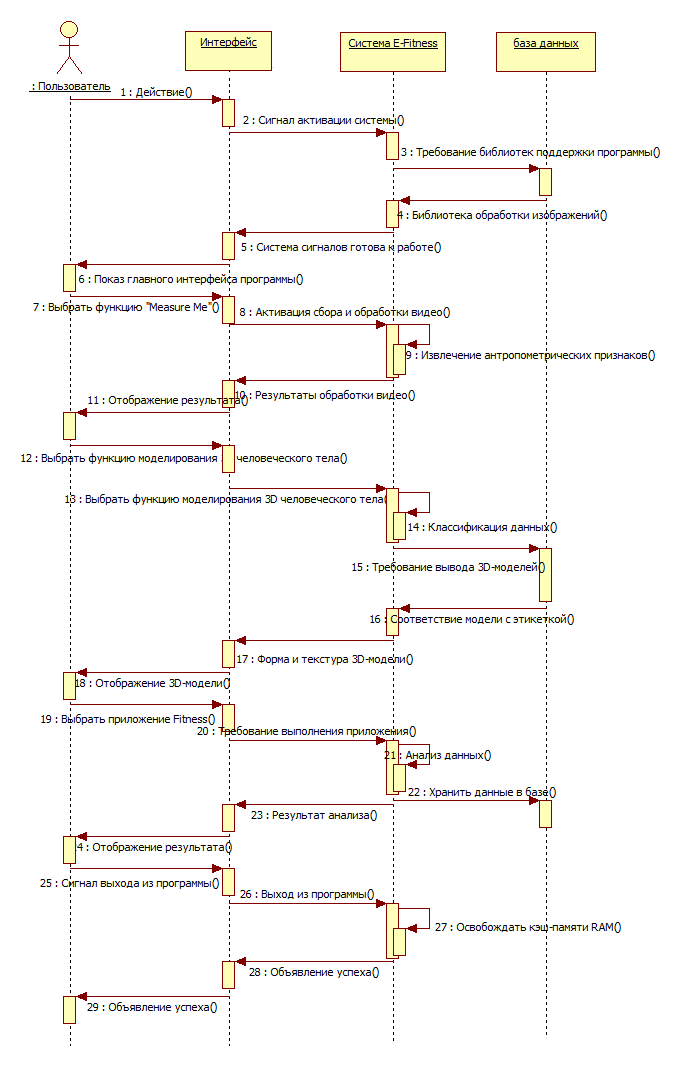
\includegraphics[width=0.45\linewidth]{p18}
\begin{center}
%\captionsetup{justification=justified, labelsep=period}
\caption{Диаграмма последовательности - система компьютерного зрения в антропометрии приложения E- Fitness.}
\end{center}
\end{figure}
\end{frame}
%-----------------------------------------------------------
\begin{frame}{Применение системы компьютерного зрения в антропометрии для пошива одежды (E-Tailor)}
\begin{columns}
		\begin{column} {0.5\textwidth}			
\textbf{Основные функции приложения E-Tailor}
\begin{itemize}
	\item Позволять пользователям добавлять информацию;
	\item Показать 3D-модель на основе антропометрических признаков и классификации данных;
	\item Позволять пользователям выбрать марки одежды и классифицировать размеры одежды.
\end{itemize}
			\end{column}
			\begin{column} {0.5\textwidth}
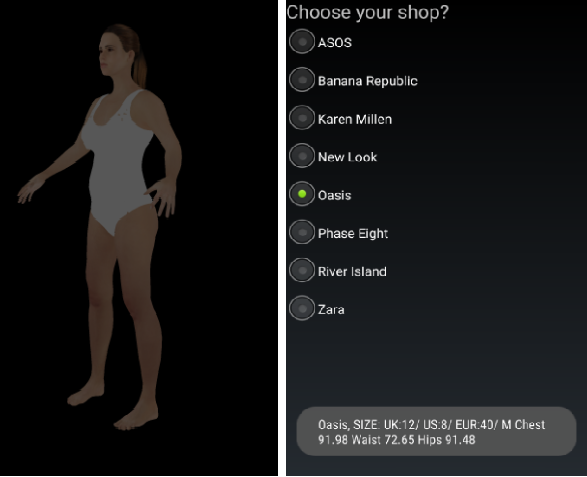
\includegraphics[width=1\linewidth]{p19}
			\end{column}      
		\end{columns}

\begin{center}
		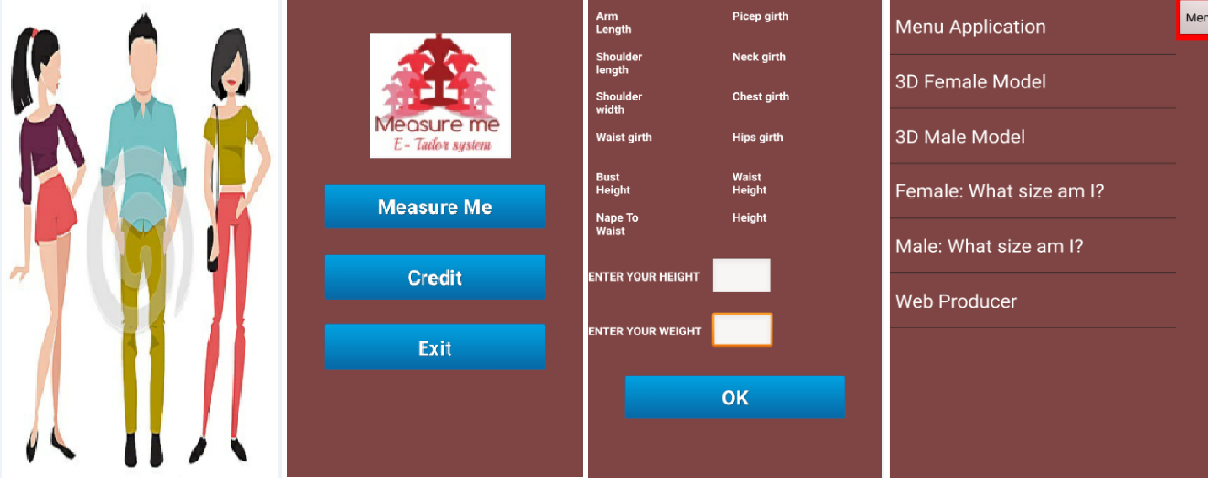
\includegraphics[width=0.5\linewidth]{p20}
\end{center}

\end{frame}
%-----------------------------------------------------------
\begin{frame}{Применение системы компьютерного зрения в антропометрии для фитнеса (E-Fitness)}
\begin{columns}
		\begin{column} {0.5\textwidth}			
\textbf{Основные функции приложения E-Fitness}
\begin{itemize}
	\item Позволять пользователям добавлять информацию;
	\item Показать 3D-модель на основе антропометрических признаков и классификации данных;
	\item Анализ антропометрических признаков на основе стандартов Fitness.
\end{itemize}
\begin{center}
		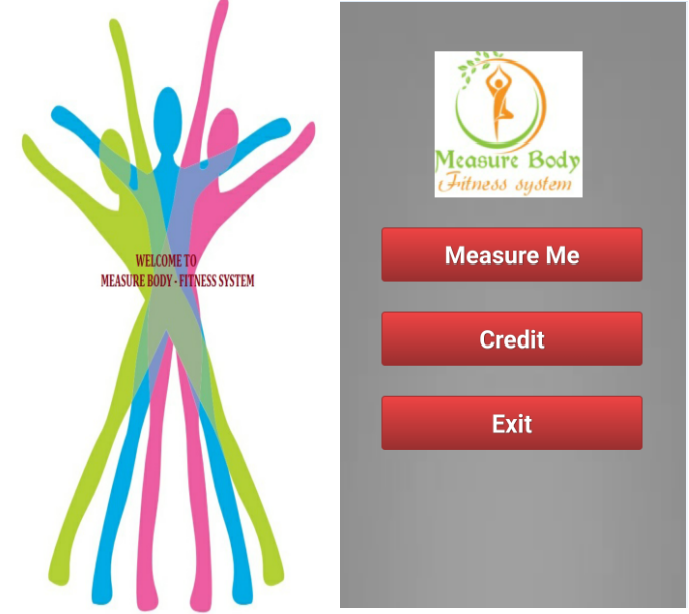
\includegraphics[width=0.5\linewidth]{p22}
\end{center}
			\end{column}
			\begin{column} {0.5\textwidth}
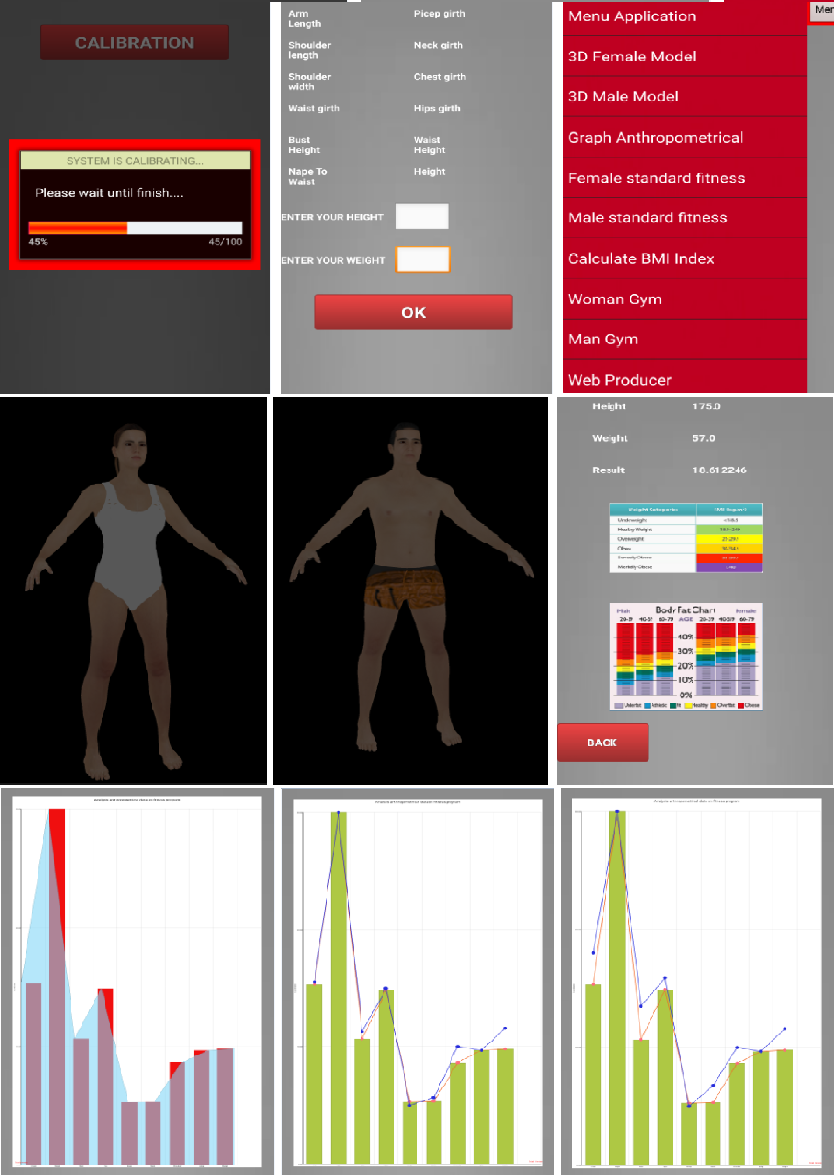
\includegraphics[width=0.85\linewidth]{p21}
			\end{column}      
		\end{columns}
\end{frame}
%-----------------------------------------------------------
\begin{frame}{ОСНОВНЫЕ РЕЗУЛЬТАТЫ И ВЫВОДЫ}
\begin{enumerate}
	\item Разработаны и применены алгоритмы компьютерного зрения для  извлечения антропометрических признаков из видеопоследовательностей на основе комбинации алгоритмов сегментации изображений разреза на графах (Graph-cuts) и итеративного алгоритма ближайших точек (ICP), построение множества ключевых точек объектов;
	\item Применен алгоритм классификации антропометрических данных методом случайного леса (Random Forest).
	\item Разработан способ построения антропометрических 3D-моделей человеческого тела на основе интеллектуального анализа антропометрических признаков;
	\item Предложенный и обоснованный подход реализован в виде приложения для смартфонов на ОС Android: приложение «E-Tailor» для текстильной промышленности и приложение «E-Fitness» для фитнеса.
\end{enumerate}

\end{frame}

%---------------------------------------------------------------------
\begin{frame}{Список публикаций по теме диссертации}
    \textbf{ВАК и Scopus/WebOfScience публикации}
		\begin{enumerate}
  \item Нгуен Тхе Лонг, Нгуен Тху Хыонг. Об автоматизации извлечения и классификации антропометрических признаков// Вестник ИРНИТУ №4 - 2015. С17-23.
	\item Нгуен Тхе Лонг, Нгуен Тху Хыонг. О распознавании и классификации дефектов дорожного покрытия на основе изображений // Вестник ИРНИТУ №10 - 2016. C111-118.
	\item Long The Nguyen, Huong Thu Nguyen, Automatic Anthropometric System
Development Using Machine Learning, BRAIN. Broad Research in Artificial
Intelligence and Neuroscience, 2016, Vol.7, pp 5-15.	
	\end{enumerate} 
\textbf{Свидетельство о государственной регистрации программы для ЭВМ:}
			\begin{enumerate}
			\item  Свидетельство № 2016611475 от 03.02.2016 о государственной регистрации программы для ЭВМ. Программа бесконтактной антропометрии для смартфонов на операционной системе Андроид // Сидоров Д.Н., Нгуен Т.Л., Нгуен Т.Х.
	\item  Свидетельство № 2016619386 от 18.08.2016 о государственной регистрации программы для ЭВМ. Программа бесконтактной антропометрии для смартфонов на операционной системе Андроид // Сидоров Д.Н.,  Нгуен Т.Х., Нгуен Т.Л.
	\end{enumerate} 	
		\end {frame}
		%%%%%%%%%%%%%%
	\begin{frame}{Свидетельство программы ЭВМ}	 

\begin{center}
     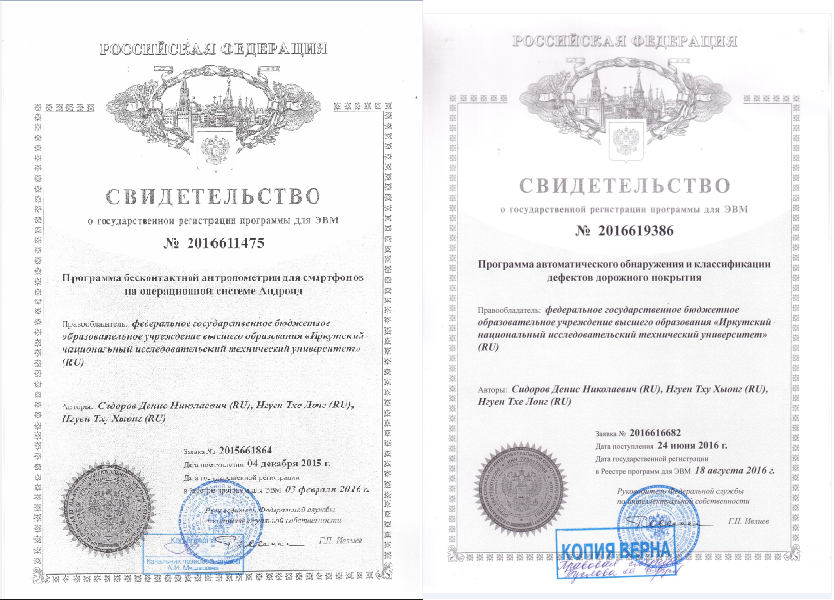
\includegraphics[width=1\linewidth]{p23}
\end{center}

			\end{frame}		
			%%%%%%%%%%%%%%
		\begin{frame}{Другие публикации}
		\begin{itemize}
  \item Нгуен Тхе Лонг, Нгуен Тху Хыонг. Автоматизация антропометрических измерений и извлечение признаков из 2D-изображений// Байкалская международная школа-семинар "Методы оптимизации и их приложения". О. Ольхон, Иркутск 2014г. С 153.
	\item Нгуен Тхе Лонг, Нгуен Тху Хыонг. Построение программы для обнаружение контуров человека в изображении с помощью методов математической морфологии// Материалы всероссийской молодежной научно-практической конференции «Винеровские чтения 2014». Иркутск: Изд-во Иркутск, 2014. Стр.10.
	\item Нгуен Тхе Лонг, Нгуен Тху Хыонг. Методы математической морфологии в цифровой обработке изображений// Труды XIX Байкальской Всероссийской конференции «информационные и математические технологии в науке и управлении». Иркутск: ИСЭМ СО РАН, 2014. С75-81.
		\end{itemize}
		\end{frame}
		\begin{frame}{Другие публикации}
		\begin{itemize}
	\item Нгуен Тхе Лонг. Классификация и кластерный анализ антропометрических признаков// Материалы всероссийской молодежной научно-практической конференции «Винеровские чтения 2015». Иркутск: Изд-во Иркутск, 2015. Стр.8.
	\item Нгуен Тхе Лонг, Нгуен Тху Хыонг. Анализ с использованием методов машинного обучения// Междисциплинарные исследования в области математического моделирования и информатики. Ульяновск: Изд-во SIMJET, января 2015г. С204-210.
	\item Nguyen The Long, Nguyen Thu Huong, Aleksei Zhukov. Anthropometrical Features using Machine Learning Approach// Supplementary Proceedings of the 4th International Conference on Analysis of Images, Social Networks and Texts (AIST'2015). CEUR Workshop Proceedings. Page 96-105.
	 	\end{itemize}
\end{frame}
%---------------------------------------------------------------------
\begin{frame}{Акты}	 
\begin{center}
     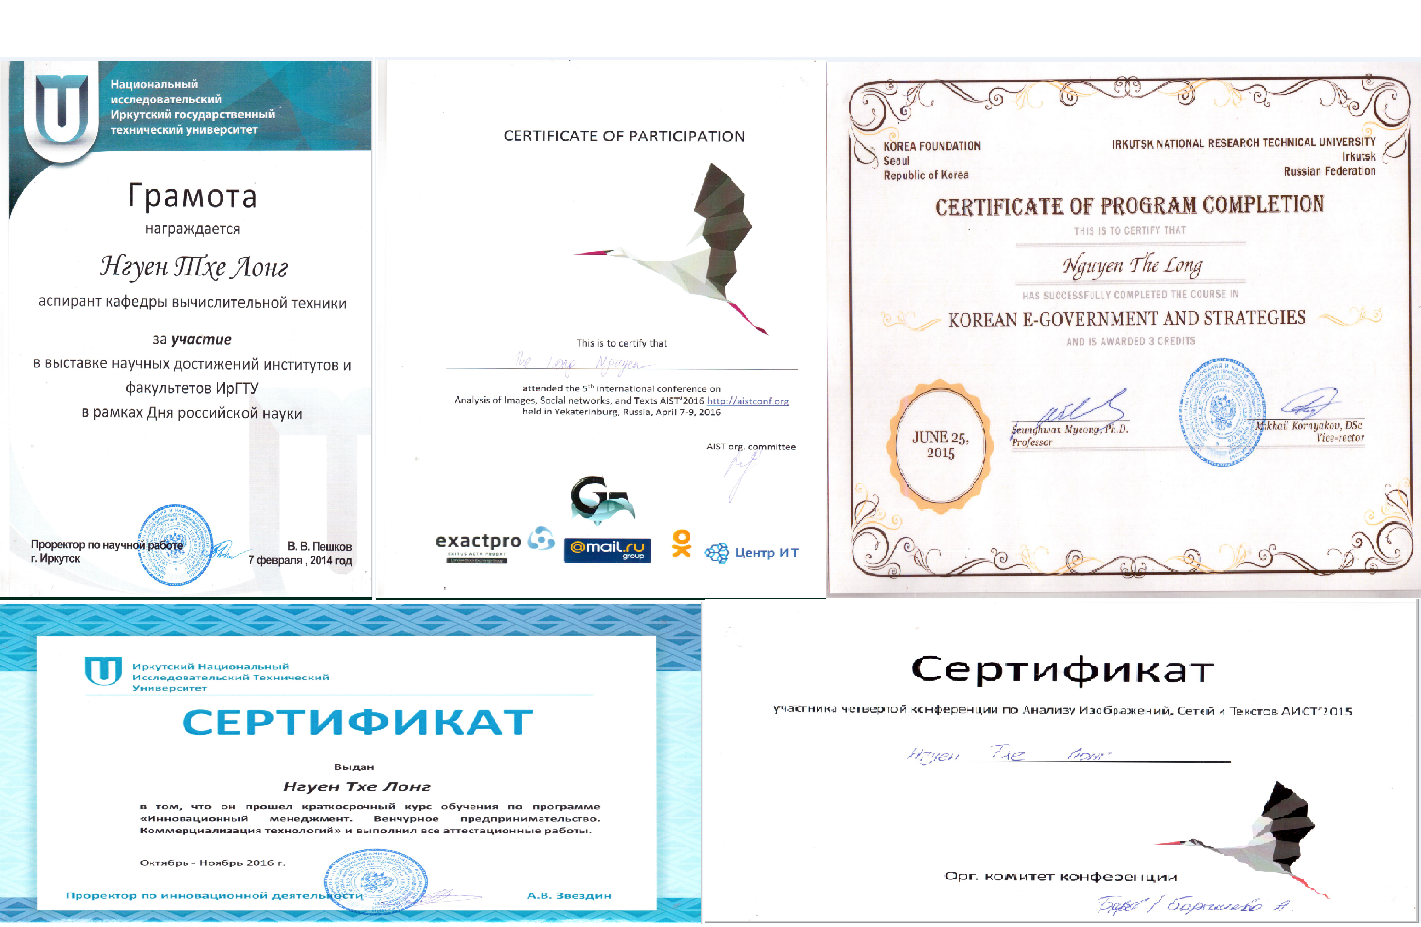
\includegraphics[width=1\linewidth]{p24}
\end{center}
			\end{frame}
%-----------------------------------------------------------
\begin{frame}[fragile]
  \frametitle{}
\textcolor[rgb]{1,0,0}{\Huge{\centerline{ Спасибо за внимание!}}   } 
\end{frame}
%---------------------------------------------------------------------

\end{document}